\documentclass{article}
\usepackage{epsfig, latexsym}

\begin{document}

\newcommand{\bs}{\backslash}

\title{
\Large{CMPEN 271 -- Fall 2010}\\
\normalsize{Exam 2}\\
\makebox[4in][l]{Name:} 
PSU ID:}
\date{}
\maketitle{}

\begin{enumerate}
\item {\bf (3 pts.)} Assuming a word size of 5 bits, interpret 10110 
as a 2's complement number.

\begin{tabular}{p{0.6in} p{0.6in} p{0.6in} p{0.6in} l}
a) -9 & b) -10 & c) -5 & d) 22 & e) None of the above.
\end{tabular}

\item {\bf (3 pts.)} Assuming a word size of 5 bits, determine the 2's complement
representation of -9.

\begin{tabular}{p{0.6in} p{0.6in} p{0.6in} p{0.6in} l}
a) 11011 & b) 10111 & c) 10110 & d) 11001 & e) None of the above.
\end{tabular}

\item {\bf (4 pts.)} How many inputs do the AND gates in a 32:1 mux have?
\begin{tabular}{p{0.6in} p{0.6in} p{0.6in} p{0.6in} l}
a) 5 & b) 6 & c) 31 & d) 32 & e) None of the above.
\end{tabular}

\item {\bf (3 pts.)} How many 2:1 muxes does it take to build a 32:1 mux?

\begin{tabular}{p{0.6in} p{0.6in} p{0.6in} p{0.6in} l}
a) 3 & b) 7 & c) 15 & d) 31 & e) None of the above.
\end{tabular}

Questions 5-7 concern the construction of a bit-slice of a comparator.  
The questions will ask you to complete the entries in the truth table 
below denoted by $a$, $b$, and $c$.

\begin{tabular}{l|l|l|l|l||l|l|l}
$G_{in}$ & $L_{in}$ & $E_{in}$ & $x$ & $y$ & $G_{out}$ & $L_{out}$ & $E_{out}$ \\ \hline
    0    &    0     &     1    &  1  &  1  &   $a$     &           &  \\ \hline
    1    &    0     &     0    &  0  &  1  &           &   $b$     &  \\ \hline
    1    &    0     &     1    &  1  &  0  &           &           &  $c$    \\
\end{tabular}

\item {\bf (2 pts.)}What is the value of $a$?

\begin{tabular}{p{0.6in} p{0.6in} p{0.6in}}
a) 0 & b) 1 & c) x 
\end{tabular}

\item {\bf (2 pts.)}What is the value of $b$?

\begin{tabular}{p{0.6in} p{0.6in} p{0.6in}}
a) 0 & b) 1 & c) x 
\end{tabular}

\item {\bf (2 pts.)}What is the value of $c$?

\begin{tabular}{p{0.6in} p{0.6in} p{0.6in}}
a) 0 & b) 1 & c) x 
\end{tabular} \\

\pagebreak
You are given the following 4:16 decoder built from 2:4 decoders.
Unfortunately, the student who built it wired the select lines in a
most unusual fashion.  Its your job to label each output with the
index which selects it.  Most of the outputs have been omitted
for clarity.

\scalebox{0.5}{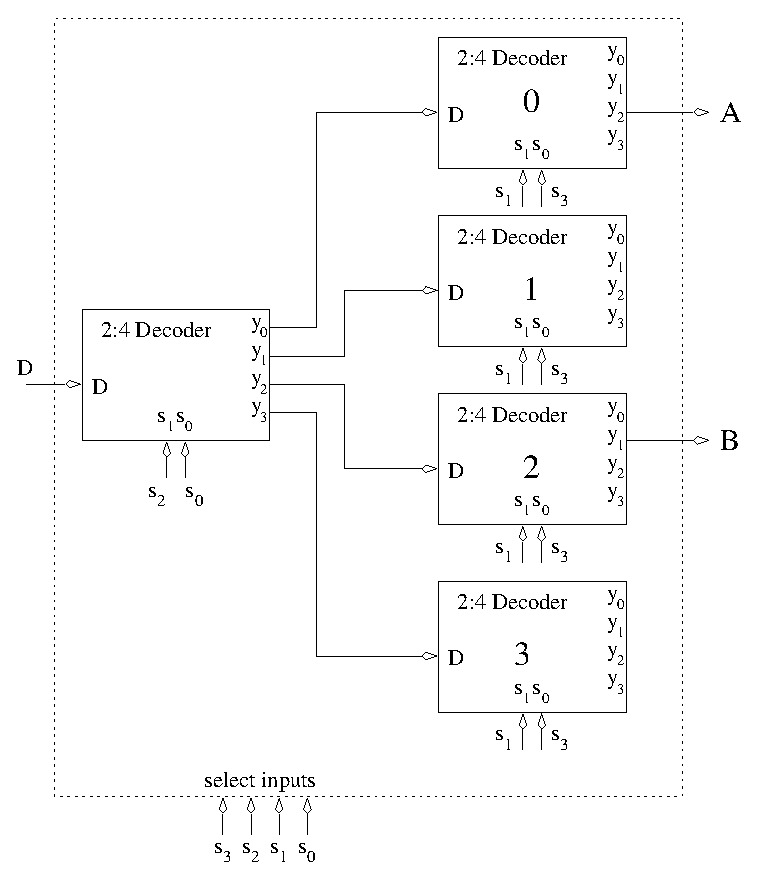
\includegraphics{./Fig2/OddDecoder}}

\item {\bf (3 pts.)} What is the value of the output labeled A?

\begin{tabular}{p{0.6in} p{0.6in} p{0.6in} p{0.6in} l}
a) $y_{1}$ & b) $y_{2}$ & c) $y_{4}$ & d) $y_{8}$ & e) None of the above
\end{tabular}

\item {\bf (3 pts.)} What is the value of the output labeled B?

\begin{tabular}{p{0.6in} p{0.6in} p{0.6in} p{0.6in} l}
a) $y_{1}$ & b) $y_{6}$ & c) $y_{9}$ & d) $y_{12}$ & e) None of the above
\end{tabular}


\item {\bf (5 pts.)} Which line of pseudo-code is equivlent to 
the following piece of hardware.  Y is a 4-bit binary number.

\scalebox{0.7}{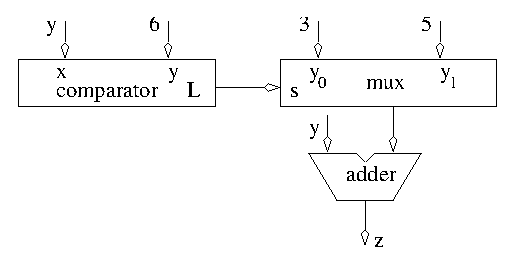
\includegraphics{./Fig2/conditional2}}

\begin{description}
\item{a) } \verb^if (5 < Y) then Z = X+3 else Z = Y+5;^
\item{b) } \verb^if (6 < Y) then Z = Y+3 else Z = Y+5;^
\item{c) } \verb^if (6 > Y) then Z = X+3 else Z = Y+5;^
\item{d) } \verb^if (5 > Y) then Z = Y+3 else Z = Y+5;^
\end{description}

\pagebreak
You have a digital design which calls for a circuit which performs the 
following task (written as a C if/then statement).  You have decided on 
the architecture.  Its your job to design to complete the truth table
for the the glue-logic box (only an arbitrary portion of the complete 
truth table is shown).  

\begin{verbatim}
if      (sum > 18) z = sum-18
else if (sum > 12) z = sum-12
else if (sum > 6)  z = sum-6
else               z = sum
\end{verbatim}

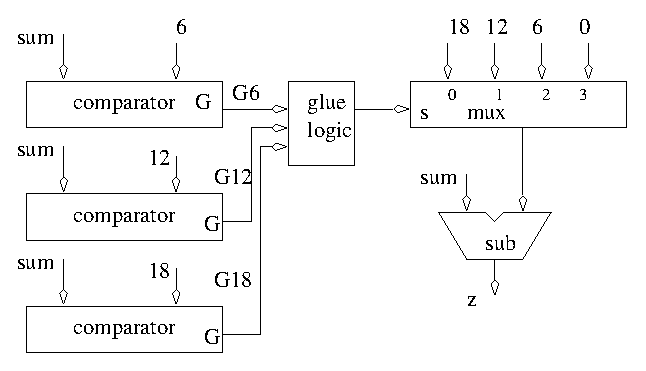
\includegraphics{./Fig2/if7}

\vspace{0.25in}

\begin{tabular}{l|l|l||l}
G6 & G12 & G18 & select \\ \hline
0  & 0   & 0   &   a   \\ \hline
1  & 1   & 0   &   b   \\ \hline
1  & 0   & 1   &   c   \\ 
\end{tabular}

\vspace{0.25in}

\item {\bf (3 pts.)}What is the (decimal) value of a in the truth table?

\begin{tabular}{p{0.6in} p{0.6in} p{0.6in} p{0.6in} l}
a) 0 & b) 1 & c) 2 & d) 3 & e) x  
\end{tabular}

\item {\bf (3 pts.)}What is the (decimal) value of b in the truth table?

\begin{tabular}{p{0.6in} p{0.6in} p{0.6in} p{0.6in} l}
a) 0 & b) 1 & c) 2 & d) 3 & e) x  
\end{tabular}

\item {\bf (3 pts.)}What is the (decimal) value of c in the truth table?

\begin{tabular}{p{0.6in} p{0.6in} p{0.6in} p{0.6in} l}
a) 0 & b) 1 & c) 2 & d) 3 & e) x  
\end{tabular}

\pagebreak
\begin{tabular}{llll}
\begin{tabular}{c||c}
D & Q+   \\ \hline
0 & 0 \\ \hline
1 & 1 \\
\end{tabular}
&
\begin{tabular}{c||c}
T & Q+   \\ \hline
0 & Q \\ \hline
1 & Q' \\
\end{tabular}
&
\begin{tabular}{c|c||c}
S & R & Q+   \\ \hline
0 & 0 & Q \\ \hline
0 & 1 & 0 \\ \hline
1 & 0 & 1 \\ \hline
1 & 1 & x \\
\end{tabular}
&
\begin{tabular}{c|c||c}
J & K & Q+   \\ \hline
0 & 0 & Q \\ \hline
0 & 1 & 0 \\ \hline
1 & 0 & 1 \\ \hline
1 & 1 & Q' \\
\end{tabular}
\end{tabular}

\underline{For questions 14-19 use the following figure.}
Assume that initial value of Q is 0 (as shown in the figure),
and that the outputs, after a period of rapid toggling, 
end-up at 0.

\scalebox{0.7}{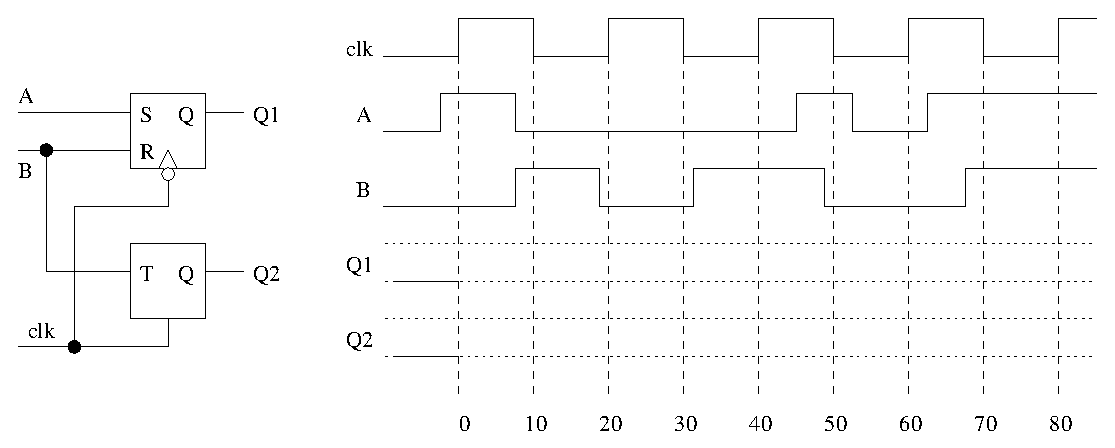
\includegraphics{./Fig2/ExTim4}}

\item {\bf (3 pts.)} What is the value of Q1 at time 25

\begin{tabular}{p{0.75in}p{0.75in}p{0.75in}p{1.25in}}
a) 0 & b) 1 & c) toggling & d) unknown \\
\end{tabular}

\item {\bf (2 pts.)} What is the value of Q1 at time 35

\begin{tabular}{p{0.75in}p{0.75in}p{0.75in}p{1.25in}}
a) 0 & b) 1 & c) toggling & d) unknown \\
\end{tabular}

\item {\bf (1 pt.)} What is the value of Q1 at time 65

\begin{tabular}{p{0.75in}p{0.75in}p{0.75in}p{1.25in}}
a) 0 & b) 1 & c) toggling & d) unknown \\
\end{tabular}

\item {\bf (2 pts.)} What is the value of Q2 at time 25

\begin{tabular}{p{0.75in}p{0.75in}p{0.75in}p{1.25in}}
a) 0 & b) 1 & c) toggling & d) unknown \\
\end{tabular}

\item {\bf (1 pts.)} What is the value of Q2 at time 45

\begin{tabular}{p{0.75in}p{0.75in}p{0.75in}p{1.25in}}
a) 0 & b) 1 & c) toggling & d) unknown \\
\end{tabular}

\pagebreak
For problems 19-23 use the following figure and timing diagram.
You should assume that all the devices process 5-bits data
values.

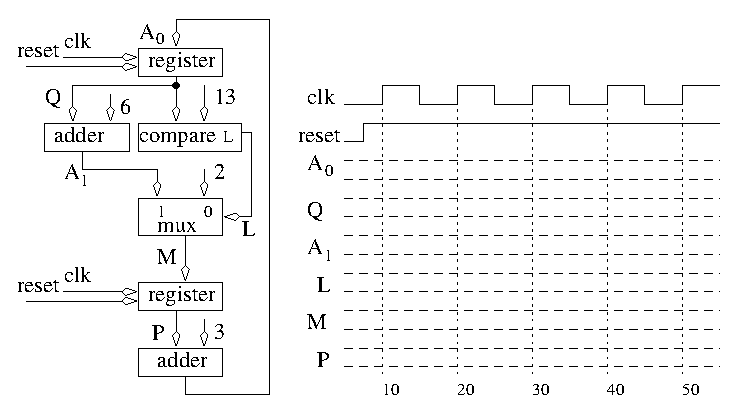
\includegraphics{./Fig2/BBBtiming4}

\item {\bf (5 pts.)}What is the value of $Q$ at time 15?

\begin{tabular}{p{0.6in} p{0.6in} p{0.6in} p{0.6in} l}
a) 0 & b) 3 & c) 6 & d) 9 & e) none of the above
\end{tabular}

\item {\bf (4 pts.)}What is the value of $P$ at time 25?

\begin{tabular}{p{0.6in} p{0.6in} p{0.6in} p{0.6in} l}
a) 2 & b) 9 & c) 12 & d) 15 & e) none of the above
\end{tabular}

\item {\bf (3 pts.)}What is the value of $A_1$ at time 35?

\begin{tabular}{p{0.6in} p{0.6in} p{0.6in} p{0.6in} l}
a) 5 & b) 9 & c) 12 & d) 18 & e) none of the above
\end{tabular}

\item {\bf (2 pts.)}What is the value of $M$ at time 45?

\begin{tabular}{p{0.6in} p{0.6in} p{0.6in} p{0.6in} l}
a) 2 & b) 5 & c) 11 & d) 12 & e) none of the above
\end{tabular}

\item {\bf (1 pts.)}What is the value of $Q$ at time 55?

\begin{tabular}{p{0.6in} p{0.6in} p{0.6in} p{0.6in} l}
a) 5 & b) 11 & c) 12 & d) 14 & e) none of the above
\end{tabular}
\end{enumerate}
\end{document}
